% Rules for the HuroCup Soccer Competition
% Jacky Baltes <jacky@cs.umanitoba.ca> 

\documentclass[12pt]{hurocup}

\newcommand{\thisyear}{2010}

\newcommand{\HuroCup}{\textsc{HuroCup}}


\begin{document}

\title{\HuroCup: Soccer\\
Laws of the Game \thisyear}

\author{Jacky Baltes\\
Autonomous Agents Laboratory\\
University of Manitoba\\
Winnipeg, Manitoba\\
Canada, R3T 2N2\\
Email: jacky@cs.umanitoba.ca\\
WWW: http://www.cs.umanitoba.ca/\~{ }jacky\\[5mm]
Kuo-Yang Tu\\
National Kaohsiung First University of Science and Technology\\
Kaohsiung City, R. O. C.\\
Email: tuky@ccms.nkfust.edu.tw\\
}

\maketitle
\begin{abstract}
The following rules and regulations govern the soccer event in
\HuroCup, a robotic game and robotics benchmark problem for humanoid
robots.
%
\end{abstract}

\section*{Latest Version of the Rules for \HuroCup}
\label{sec:updates}

The latest official version of the rules of the game for \HuroCup\ is
always available from the FIRA \HuroCup\ website (http://www.fira.net).

\newpage

\section{Soccer}
\label{sec:soccer}

The following rules govern the game of 3 vs 3 soccer in the \HuroCup\
competition. The rules are based on the FIRA rules as well as the FIFA
rules.

Since soccer is a team event, it puts more stress on the already
limited resources of many humanoid robotic teams. Teams that are not
able to field a full team of players are therefore encouraged to join
forces with other teams in a similar situation. Teams are encouraged
to inform the organizing committee before the competition if they are
planning on forming a joint team or are looking for partner teams, so
that the organizing committee can get teams in touch with other
teams. However, the teams may be formed during the \HuroCup\
competition until the first game in the soccer event is started.

\section{Laws of the Game}
\label{sec:laws}

The following laws are intended for humanoid robot soccer. As such,
they provide a background and further information for the laws of the
individual events.

\law{The Field of Play}
\label{law:field-of-play}

\begin{lawlist}
  
\item The playing surface is a hardwood surface or a carpet. The floor
  under the surface is level, flat and hard.

\item The color of the playing field is matt black or green.
  
\item Dimensions: The length of the field must be rectangular. The
  length of the field (touch line) must be greater than the width of
  the field (goal line). The length of the field must be greater than
  340cm and less than 430cm. The width of the field must be greater
  than 250cm and less than 350cm.
 
\item There is a 30cm wide boundary around the playing field. The
  boundary area is \emph{not} part of the playing field. Its purpose
  is to prevent damage to robots leaving the playing field.
 
\item The field of play is marked with lines. These lines belong to
  the area of which they are boundaries. The two longer boundary lines
  are called touch lines. The two shorter ones are called goal lines.

\item All lines are marked in white color and are not more than 5mm
  wide. 

\item The field of play is divided into two halves by a half way
  line. 

\item The center mark is indicated at the midpoint of the half way
  line. A circle with a diameter of 100cm is marked around it.
  
\item A figure of one possible legal playing field is shown in
  Fig.~\ref{fig:field-hurocup}.
  
  \begin{figure}
    \begin{center}
      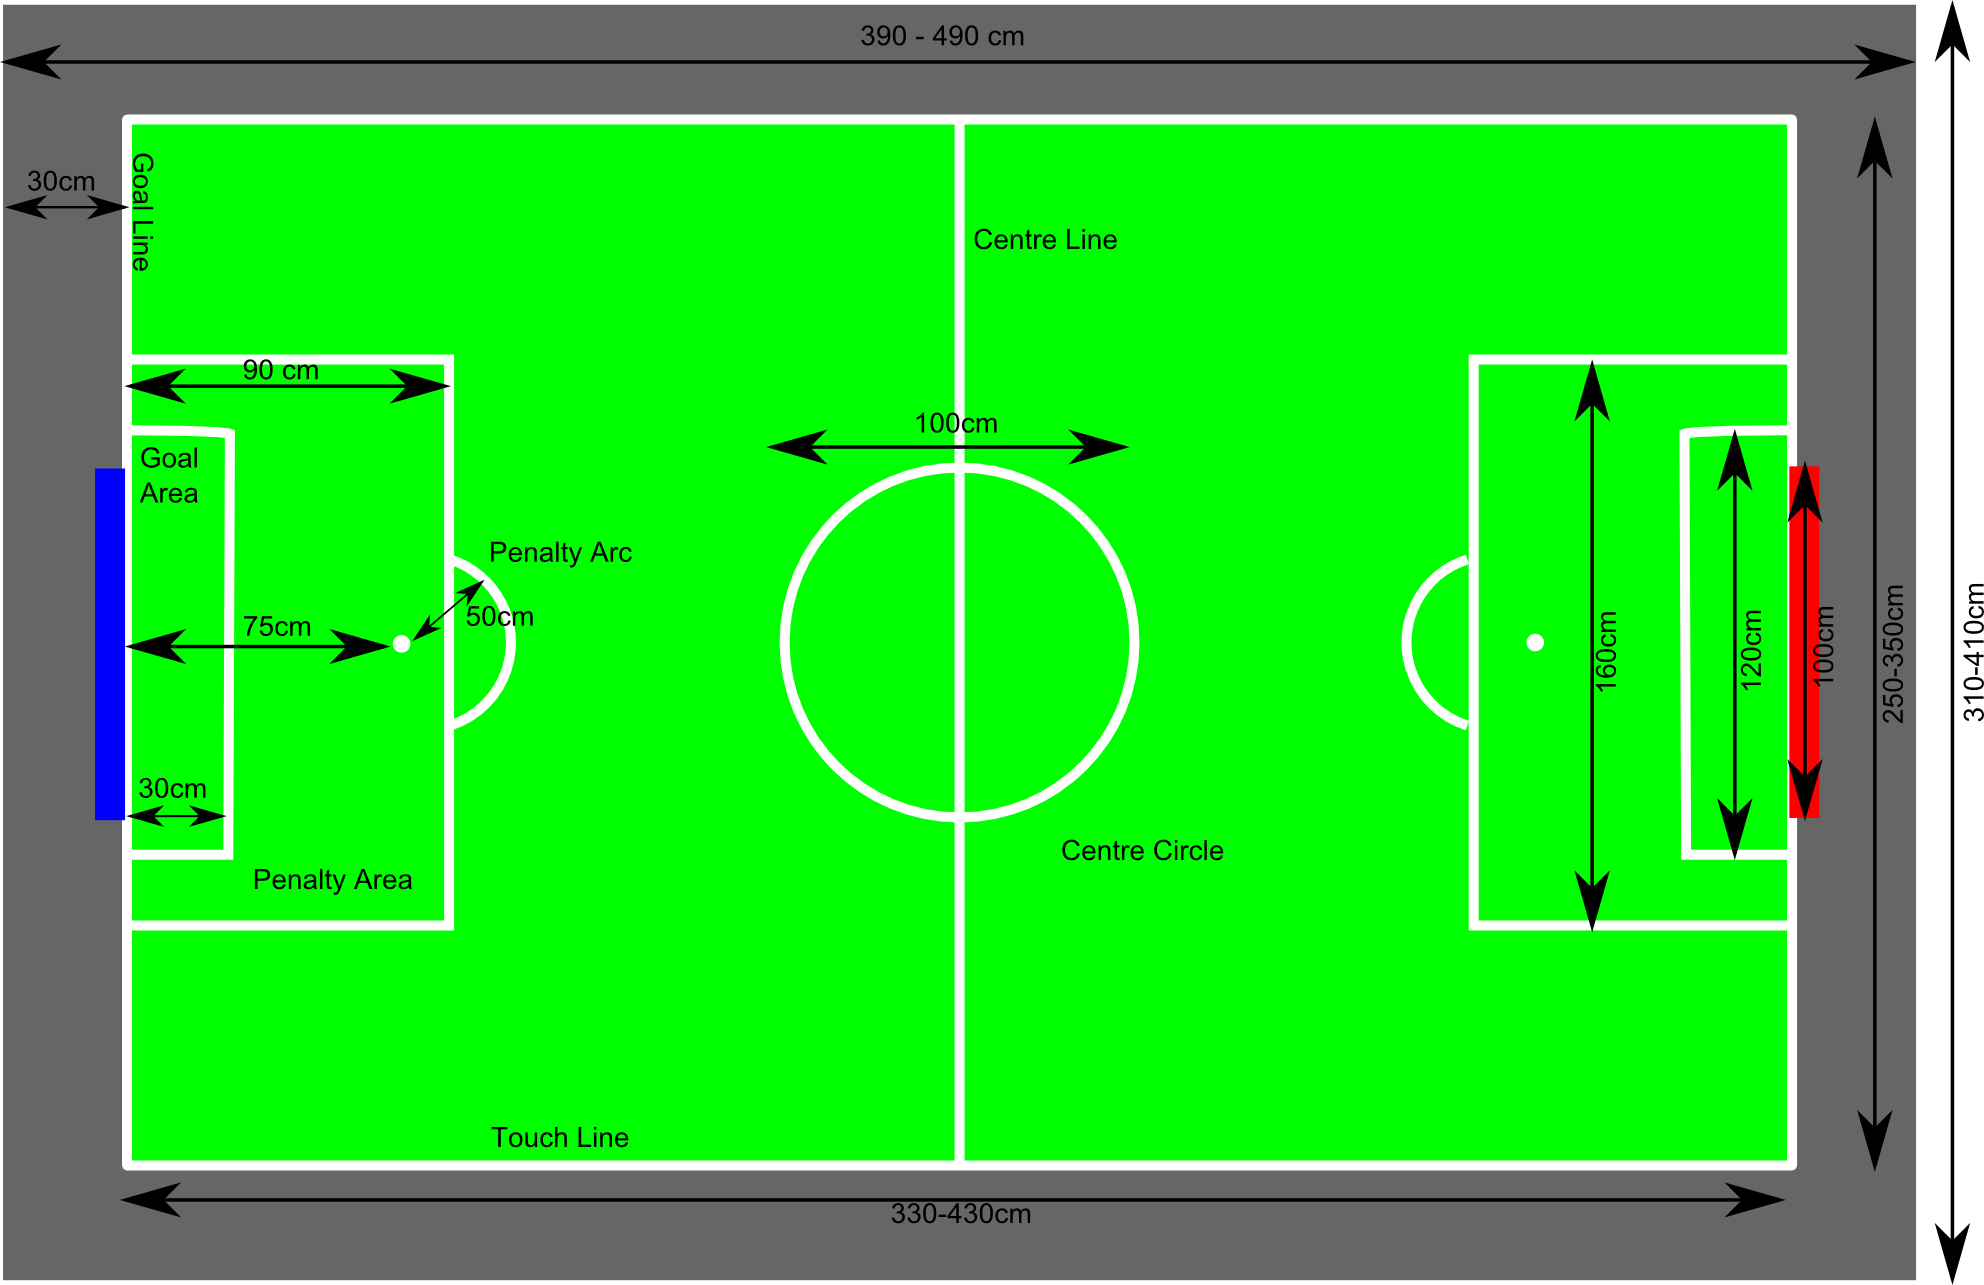
\includegraphics[width=0.8\textwidth]{Figures/hurocup-field}
      \caption{The field of play for \HuroCup}
      \label{fig:field-hurocup}
    \end{center}
  \end{figure}
  
\item Goal Area: A goal area is defined at each end of the field as
  follows: Two lines are drawn at right angles to the goal line, 10cm
  from the inside of each goalpost. These lines extend into the field
  of play for a distance of 30cm and are joined by a line drawn
  parallel with the goal line. The area bounded by these lines and the
  goal line is the goal area.
  
\item Penalty Area: A penalty area is defined at each end of the field
  as follows: Two lines are drawn at right angles to the goal line,
  30cm from the inside of each goalpost. These lines extend into the
  field of play for a distance of 90cm and are joined by a line drawn
  parallel with the goal line. The area bounded by these lines and the
  goal line is the penalty area.
  
\item \label{penalty-mark} Penalty Mark: Within each penalty area, a
  penalty mark is made 75cm from the midpoint between the goalposts
  and equidistant to them.
  
\item \label{penalty-arc} Penalty Arc: The arc outside of the penalty
  area of the circle centered on the penalty mark and with a radius of
  50cm is drawn.

\item Goals must be placed on the center of each goal line. They
  consist of two upright posts equidistant from the corner flag posts
  and joined at the top by a horizontal crossbar.
  
\item The distance between the posts is 100cm and the distance from
  the lower edge of the crossbar to the ground is 60cm. Both goalposts
  and the crossbar have the same width and depth which do not exceed 5
  cm.
  
\item Nets may be attached to the goals and the ground behind the
  goal, provided that they are properly supported and do not interfere
  with the goalkeeper.
  
\item The goal posts and crossbar of the goal on one side of the
  playing field are colored in red (the red goal).
  The goal posts and crossbar of the goal on the other side are
  colored in blue (the blue goal).
  
\item Goals must be anchored securely to the ground. Portable goals
  may only be used if they satisfy this requirement.

\end{lawlist}

\begin{decisions}

\item The field of play shall be lighted by natural indoor
  lighting. The lighting should be as uniform as possible. The local
  organizing committee should attempt to provide information about the
  specific lighting conditions as early as possible to the
  competitors.
  
\item The specific color and texture of the surface is not specified
  and may vary from competition to competition (just as real soccer
  fields vary). 

\item The surface underneath the carpet is level and
  hard. Examples of approved surfaces include: cement, linoleum,
  hardwood flooring, plywood, ping-pong tables and particle board;
  carpeted or cushioned surfaces are not allowed. Every effort shall
  be made to ensure that the surface is flat, however, it is up to
  individual teams to design their robots to cope with slight
  curvatures of the surface.

\end{decisions}

\law{The Ball}
\label{law:ball}

\begin{lawlist}
\item Robots in the \textit{small} category shall be using a yellow
 tennis ball.

\item Robots in the large category shall use an orange youth (Size 3)
soccer ball. 

\item If the ball becomes defective during the course of a match:
  \begin{itemize}
  \item the match is stopped,
  \item the match is restarted by placing the replacement ball at the place where the first ball became defective, 
  \item if the ball becomes defective whilst not in play at a
    kick-off, goal kick, corner kick, free kick, penalty kick or
    throw-in, then the match is restarted accordingly,
  \end{itemize}
\item the ball may not be changed during the match without the authority of the referee.

\end{lawlist}

\law{Number of Robots}

\begin{lawlist}
\item A match is played with two teams, each consisting of not more
  than three players in the small category, and not more than two
  players for robots in the large category. One of the robots on a
  team is the goal keeper.
\item A maximum of two substitutes may be used in a game.
\end{lawlist}

\law{Method for Scoring}
\label{law:scoring}

\begin{lawlist}
  
\item A goal is scored when the whole of the ball passes over the goal
  line, between the goal walls, below the crossbar, provided that no
  infringement of the Laws of the Game has been committed previously
  by the team scoring the goal.
  
\item The team scoring the greater number of goals during a match is
  the winner. If both teams score an equal number of goals, or if no
  goals are scored, the match is a draw.
  
\item For matches ending in a draw, competition rules may state
  provisions involving extra time, or other procedures approved by the
  local organizing committee to determine the winner of a match.
\end{lawlist}

\law{Fouls and Misconduct}
\label{law:penalties}

\begin{lawlist}
\item Cautionable Offenses: A team is cautioned and shown the yellow
  card if a robot on that team commits any of the following eight
  offenses:
  \begin{enumerate}
  \item pushes an opponent
  \item holds an opponent
  \item strikes or attempts to strike an opponent
  \item charges an opponent
  \item damages or causes likely damage to another robot
  \item is guilty of unsporting behavior
  \item modifies or damages the field, goal, or ball
  \item persistently infringes the Laws of the Game
  \end{enumerate}
\item Sending-Off Offenses: One robot is sent off and shown the red
  card if his team receives a second caution. The number of players on
  the team is reduced by one after every two yellow cards.
\end{lawlist}

\begin{decisions}
\item It is the intention of the rules committee to disallow any
  and all contact with other players. Controlled or uncontrolled
  contact must be avoided, especially in the humanoid league where
  robots are not very stable (yet!).
\end{decisions}

\law{Penalty Kick}
\label{law:penalty-kick}

\begin{lawlist}
  
\item A penalty kick is awarded if any of the seven offenses for which
  a penalty kick may be awarded is committed by a robot inside his own
  penalty area, irrespective of the position of the ball, provided it
  is in play.
  
\item A goal may be scored directly from a penalty kick.
  
\item Additional time is allowed for a penalty kick to be taken at the
  end of each half or at the end of periods of extra time.
  
\item Procedure for a Penalty Kick: A penalty kick is taken by
  following this sequential procedure.
  \begin{enumerate}
  \item The ball is placed on the penalty mark
  \item  The defending goalkeeper is positioned so that some part of
    its construction touches the goalmouth line, facing the kicker,
    until the referee gives the start signal.
  \item The defending goal keeper must remain in a standard walking
    posture until the ball is kicked.
  \item The robot taking the penalty kick is: 
    \begin{itemize}
    \item properly identified,
    \item may be positioned by the team's designated robot handler.
    \end{itemize}
  \item The robots other than the kicker and the defending goalkeeper
    are located:
    \label{pk-other-players}
    \begin{itemize}
    \item inside the field of play,
    \item at least 15cm behind the penalty mark.
    \end{itemize}
 \item Where robots must be moved to comply with this law, the
   respective designated robot handlers may position them. The
   designated robot handler may always move the defending goalkeeper. 
 \item The Referee
   \begin{itemize}
   \item does not signal for a penalty kick to be taken until the
     robots have been placed in position in accordance with the Law,
   \item decides when a penalty kick has been completed.
   \end{itemize}
 \end{enumerate}   

\item The ball is in play when the referee signals.

\item When a penalty kick is taken during the normal course of play,
  or time has been extended at half-time or full time to allow a
  penalty kick to be taken or retaken, a goal is awarded if the ball
  completely passes the goal line between the goalposts and under the
  crossbar.  even if the ball touches either or both of the goalposts
  and/or the crossbar, and/or the goalkeeper.

\item Infringements/Sanctions: \label{pk-infringements} If the referee gives the signal for a
  penalty kick to be taken and, before the ball is in play, one of the
  following situations occurs:

  The player taking the penalty kick infringes the Laws of the Game:
  \begin{itemize}
  \item the referee allows the kick to proceed,
  \item if the ball enters the goal, the kick is retaken,
  \item if the ball does not enter the goal, the kick is not retaken.
  \end{itemize}

  The goalkeeper infringes the Laws of the Game:
  \begin{itemize}
  \item the referee allows the kick to proceed,
  \item if the ball enters the goal, a goal is awarded,
  \item if the ball does not enter the goal, the kick is retaken.
  \end{itemize}

  A player of both the defending team and the attacking team
  infringe the Laws of the Game: the kick is retaken

  The ball is touched by an outside agent as it moves forward: the
  kick is retaken

  The ball rebounds into the field of play from the goalkeeper,
  the crossbar or the goalposts, and is then touched by an outside agent:
  \begin{itemize}
  \item the referee stops play,
  \item play is restarted with a dropped ball at the place where it
    touched the outside agent. 
  \end{itemize}
\end{lawlist}

\end{document}


% *** Local Variables: ***
% *** mode: LaTeX ***
% *** mode: outline-minor ***
% *** mode: auto-fill ***
% *** outline-regexp: "% !\\|\\\\\\(sub\\)*section" ***
% *** TeX-command-default: "LaTeX PDF" ***
% *** End: ***
